\documentclass{article}


\usepackage[letterpaper, margin=1in]{geometry}
\usepackage{amsmath}

\usepackage{fancyvrb} % verbatim replacement that allows latex
\DefineVerbatimEnvironment{Highlighting}{Verbatim}{commandchars=\\\{\}}

\usepackage{url}
% For basic math, align, fonts, etc.
\usepackage{amsmath}
\usepackage{amsthm}
\usepackage{amssymb}
\usepackage{mathtools}
\usepackage{mathrsfs}
\mathtoolsset{showonlyrefs}

\usepackage{hyperref}
\usepackage{siunitx}
\usepackage{float}
\usepackage{listings}

% For color
\usepackage{xcolor}
\definecolor{dark-red}{rgb}{0.4,0.15,0.15}
\definecolor{dark-blue}{rgb}{0,0,0.7}
\hypersetup{
    colorlinks, linkcolor={dark-blue},
    citecolor={dark-blue}, urlcolor={dark-blue}
}

\begin{document}

\section{Test Cases}
We have a series of test cases to ensure that our program runs correctly.
These test cases are discussed in the subsections below.
\subsection{Database Working Tests}
We have two tests for database. All these tests are in \texttt{test/db\_and\_dispatcher\_tests.py}.
\paragraph{Database Locking Test} In this test case we test that our
database is correctly locked to ensure that only one thread writes to the
files at once, hence, ensuring that the data is consistent. In this test,
we create \texttt{Cacofonix} and use dispatcher to register it to one of 
the servers. \texttt{Cacofonix} then produce a series of updates by performing
 $incrementMedalTally$ with randomly selected
teams, and medal types. There are 1000 requests of this type and
each of these requests are executed in a different thread. At the end
we retrieve the exact medal count for each team and medal type, and 
check these counts with the test's internal database to make sure that the
data retrieved is correct, hence, there is consistency in the database.

\paragraph{Update and retrieval test} 
This is the basic test used to make sure that whatever data \texttt{Cacofonix}
updates, the client is able to retrieve the exact same data. 

\subsection{Load Balancing Test}
This test is used to ensure that dispatcher indeed performs load balancing.
This test is in \texttt{test/db\_and\_dispatcher\_tests.py}. In this test,
we create twice the number of clients as the number of servers. According 
to our scheme of load balancing, it should happen that the load on each client
will be 2. At the end we check this. 


\begin{figure}[H]
        \centering
        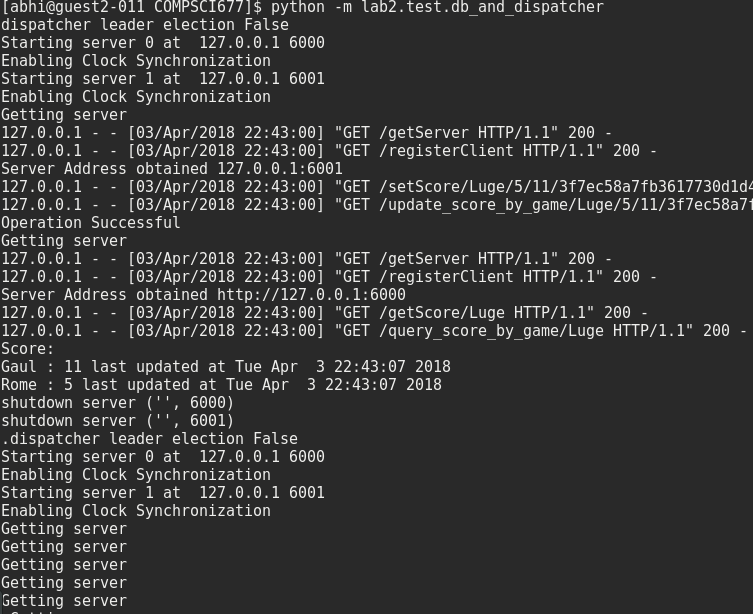
\includegraphics[width=\textwidth]{outputs/db_and_dispatcher_test_start.png}
        \caption{Clock Synchronization Start \label{fig:clong_synchronization}}
\end{figure}

\begin{figure}[H]
        \centering
        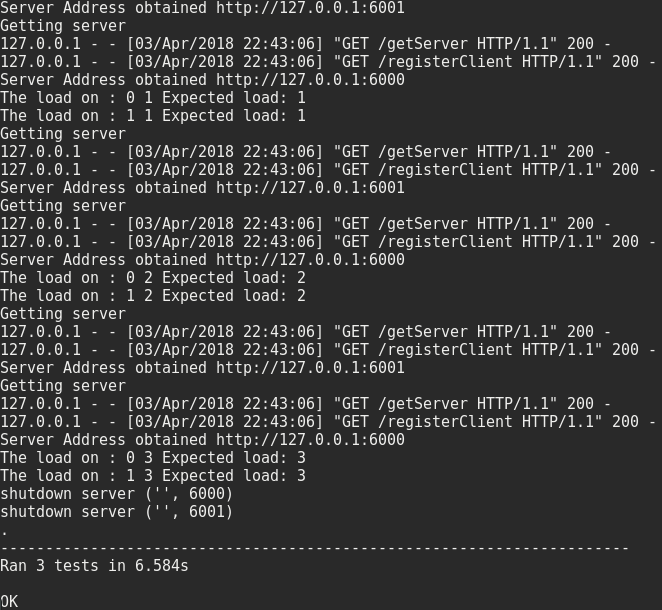
\includegraphics[width=\textwidth]{outputs/db_and_dispatcher_test_end.png}
        \caption{Totally ordered multicasting End \label{fig:clong_synchronization}}
\end{figure}


\subsection{Clock Synchronization Test}
In this test, we ensure two main properties of clock synchronization, 
(i) drift between each two servers is less than $\delta$, and (ii) the 
Berkely clock synchronization algorithm is correct. The code for this test
resides in \texttt{test/clock\_sync\_test.py}. In this test we create 2 front
end servers and 1 database server (recall that database server also takes
part in the clock synchronization). For each server we set a series of random
offsets, which has to be less than $\delta$ and store these offsets 
in an internal offsets array. We then perform the clock synchronization
10 times in both the front end servers and in the internal offsets. 
We then check that the times of each front end server matches with the internal
offset. Moreover, we also check that time difference between each clock is
less than $\delta$.

\begin{figure}[H]
        \centering
        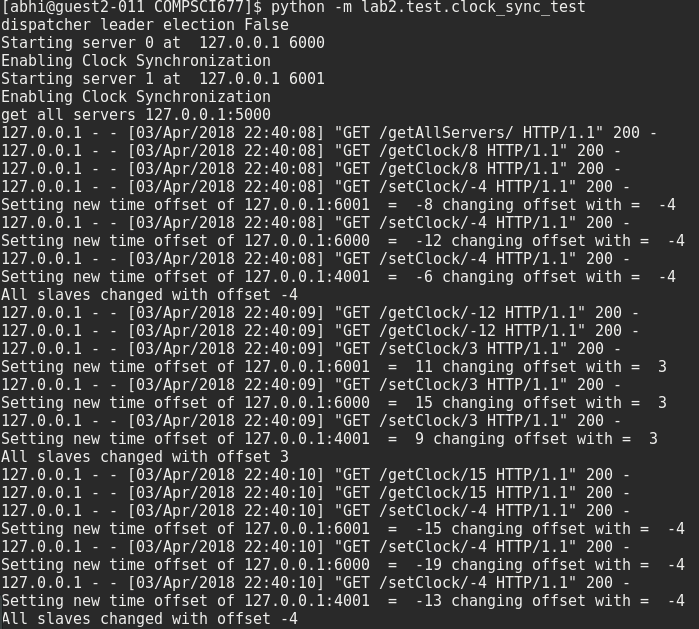
\includegraphics[width=\textwidth]{outputs/clock_sync_test_start.png}
        \caption{Clock Synchronization Start \label{fig:clonk_synchronization}}
\end{figure}

\begin{figure}[H]
        \centering
        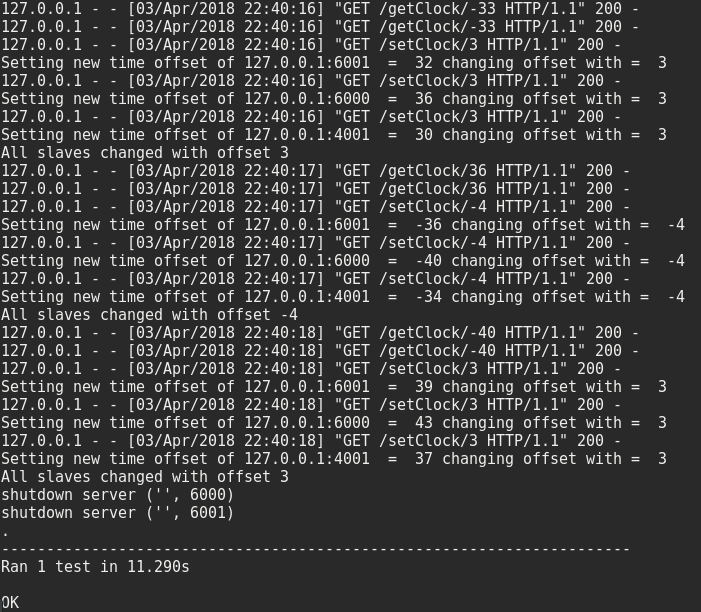
\includegraphics[width=\textwidth]{outputs/clock_sync_test_end.png}
        \caption{Clock Synchronization End \label{fig:clonk_synchronization}}
\end{figure}

\subsection{Total Multicast Ordering Test}
In this test, we ensure that the total multicast ordering is correct.
This test resides in \texttt{test/total\_ordering\_test.py}. In this test, we
first start two front end servers, and two clients. Each of the clients performs
periodic pull and sends 5 requests per second. Load Balancing of Dispatcher
ensures that each client is registered with different server. After 2 seconds
we exit the clients and shutdown the server. We then obtain all the events
obtained from each front end server in the total multicast order. We then
compare the two list of events obtained to make sure that each element of the 
list is same.

\begin{figure}[H]
        \centering
        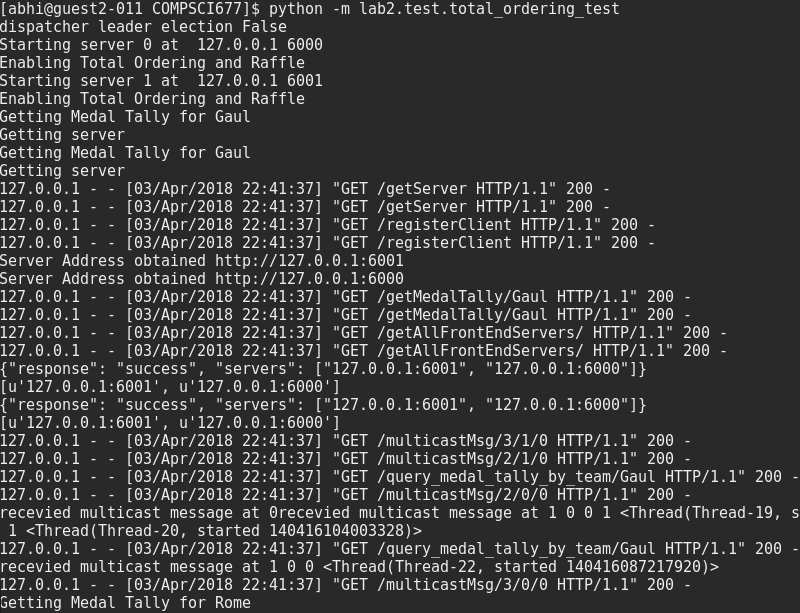
\includegraphics[width=\textwidth]{outputs/total_ordering_test_start.png}
        \caption{Clock Synchronization Start \label{fig:clong_synchronization}}
\end{figure}

\begin{figure}[H]
        \centering
        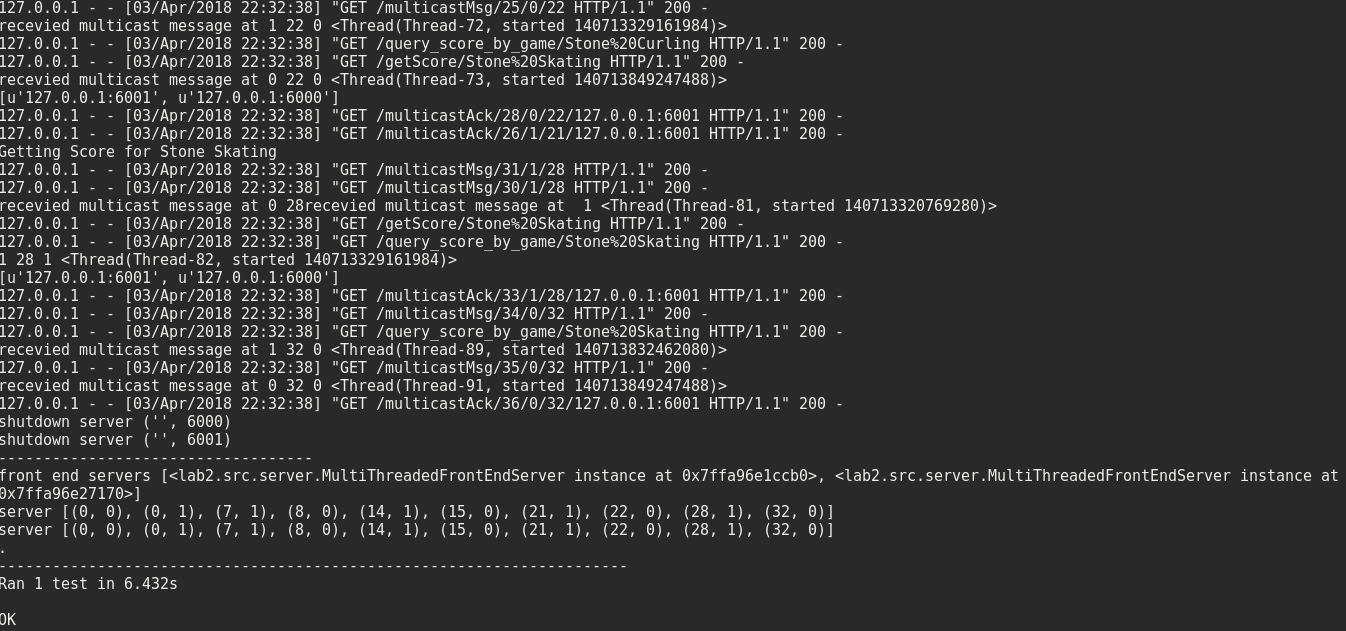
\includegraphics[width=\textwidth]{outputs/total_order_test.png}
        \caption{Totally ordered multicasting End \label{fig:clong_synchronization}}
\end{figure}



\subsection{Cases where program does not work correctly}
We do not think that there are any such cases where our program does not work
correctly.
\end{document}
